\section{System Model and Scope}


Figure~\ref{figure:model-and-decision}(a) shows the system model we are considering in this project. Endpoints (e.g., users, sensors, drones) gather and send data continuously to an instance of a Secure Real-time Decision Stack (SRDS). Endpoints can be distributed worldwide, while SRDS is typically hosted in a private or public datacenter with high connectivity to the Internet. SRDS updates a model as it receives new data from endpoints, and either pushes decisions to endpoints, or provides a pull interface to provide decisions when prompted. An example of a system pushing decisions is a navigation system that continuously updates the driving direction based on the current traffic information, while an example of a pull decision system  is a fraud detection system that makes a decision whenever a transaction is performed.

\0
\begin{figure}[h]
\center{
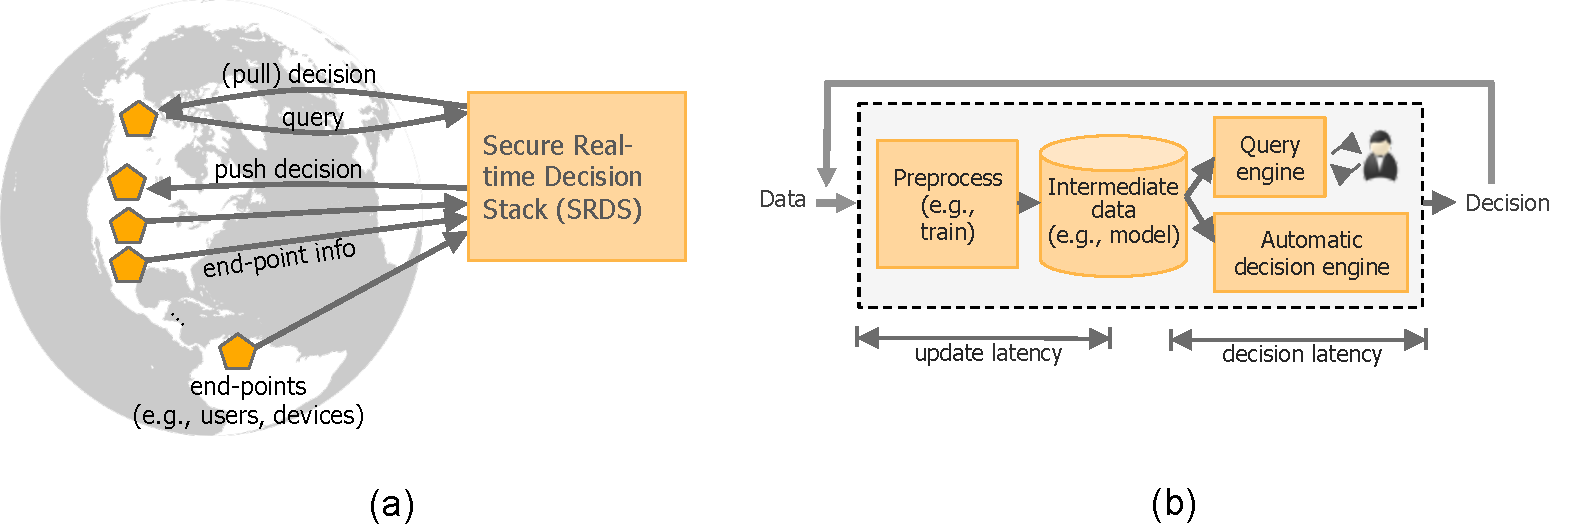
\includegraphics[scale=0.6]{figures/model-and-decision}
}
 \caption{\small{(a) High-level SRDS architecture. (b) Typical decision system.}}
  \label{figure:model-and-decision}
\end{figure}

The space of making decisions on (big) data is a huge one. Next, we summarize what is and what is not in the scope of this proposal:

\subsection{Backend vs. Endpoint Decisions}

Today, several high-profile real-time decision systems are implemented at the endpoints (e.g., self-driving cars, autonomous robots). While endpoints will remain instrumental in the decision making process, and in some cases will be the critical components of a decision system, our vision is that, going forward, more and more of the decision logic will migrate to the backend. There are several reasons for this. First, a backend engine can make decisions on the global information shared by multiple endpoints. Learning from the collective feedback of multiple endpoints can lead to better decisions than locally learning from a single endpoint. Second, a backend is much easier to scale and in general has to a much larger pool of resources than a single endpoint, which means that it can implement far more sophisticated algorithms. Finally, it is typically much easier to deploy and update software on a backend system than on endpoints. This will enable a much faster evolution of the algorithms and tools.

Of course, this will not obviate the need for endpoint-based decisions systems, or endpoints taking an active part in the decision process. Endpoints will still be the best place to implement decision algorithms for cases that require super-low latencies (e.g., self-driving cars), or that require processing huge amounts of data, such as video. However, even in those case we believe that some of the functionality will migrate to the backend or additional functionality will be deployed in the backend to augment the endpoint decisions. Examples of endpoint decision systems that will be augmented by a backend decision engine are self-driving cars sharing the information to improve driving algorithms (i.e., fleet driving), and coordinating a fleet of drones sharing the same airspace.  

For these reasons, in this proposal we will be primarily focusing on building and developing backend decision systems, such as SRDS, rather than endpoint decision systems, such as self-driving cars. This being said, we do plan to work closely with other groups at UC Berkeley and elsewhere that focus on developing endpoint decision systems, work with the community to standardize the APIs between endpoints and backend, as well as build prototypes of endpoint decision systems whenever possible.  

\subsection{Decisions vs. Actions vs. Hints}

We are using words ``decision'', ``action'', and ``hint'' interchangeably. In particular, “decision” also covers the case in which SRDS instructs an endpoint to take a particular action (e.g., changing the driving direction of an autonomous car), and the case in which it provides hints which the endpoint may choose to ignore (e.g., let a driver know about a better available route).    

\subsection{Scope of Applicability}

We have chosen to focus on supporting secure, real-time decisions on live data, as it is our belief this is the next big challenge in big data processing, and has the ability to fundamentally change the way we build intelligent systems. That being said, we expect the techniques we develop in this work to have a much broader, and even more immediate, applicability, by handling other use cases, such as decisions on historical data, high throughput interactive query workloads, low latency streaming, and secure big data processing.

At the same time, our intention is not to build a replacement for existing highly successful systems that already perform real-time decisions on live data, such as high-frequency trading and real-time ad bidding. These systems are highly-optimized for the task at hand, and, in many cases, took many years and billion dollars to build. Instead, our goal is to dramatically lower the cost and time to develop the next wave of such applications. This is similar to the way Hadoop and Spark did not target the specialized systems to index the web back in the days, but focused on democratizing big data processing, by enabling virtually everyone to build big data applications.

\section{Decision Systems}

Figure~\ref{figure:model-and-decision}(b) illustrates a simple decision system. At the high level, decisions are based on the data entering the system. In addition, the decisions can be impacted by the outcomes of the previous decisions. We call these systems ``feedback-based decision systems''.

The decision process consists of two stages. In the first stage, the raw data is transformed into an intermediate representation. A classic example of an intermediate representation is a model trained on the raw data. The second stage is where the decision actually happens. There are two types of decisions: manual and automated. With manual decisions, there is a human in the loop that queries the intermediate state (e.g., model) to make decisions, while with automated decisions there is no human in the loop.

There are two metrics that characterize the decision system performance: update latency and decision latency. The update latency determines how fast are the changes in the input data reflected in the intermediate data. The update latency determines the freshness of the model, and it is critical in a dynamic system where the model changes over time. Consider a scenario as simple as clustering tweets based on the location they originate from. As the set of active users changes, the centers of the clusters shift. As a result, the update latency can have a significant impact on the accuracy of the clustering algorithm. The decision or query latency represents the time it takes to query the intermediate data (e.g., model) in the case of human decisions, or the time it takes to make a decision in the case of automated decisions.
